\chapter{Корзины и мячи}
\label{ch:BucketsAndBalls}

Связанные данные по-прежнему в значительной степени неизвестны или неправильно поняты и недооценены. Часто людям это кажется слишком сложным. 
Поэтому я продолжаю искать новые способы сделать связанные данные более доступными. И с некоторым успехом. 
На сегодняшний момент на моих курсах более 60\% участников не имели опыта работы в области информационных технологий. Я надеюсь увеличить этот процент в будущем.

Самым сложным кажется написание SPARQL запросов. Специфика написана для ИТ-специалистов. Есть несколько отличных курсов и книг, но они также нацелены на людей с некоторым или большим опытом работы в сфере ИТ. Во всяком случае, это пугает остальных и удерживает SPARQL подальше от масс.

Я продолжаю учиться тому, что является сложным. Повторяющаяся и неожиданная проблема – это концепция переменной.

Что такое переменная в SPARQL? Просто заполнитель. Но как вы можете представить себе заполнитель? Это абстрактно. У нас нет способа постичь абстрактные вещи, если мы не ассоциируем их с чем-то физическим и конкретным. Трудно представить себе время, но как только мы рисуем его в пространстве, становится легче. Мы не можем представить мебель, но у нас нет проблем со стулом.

Другая проблема заключается в том, как выглядит запрос SPARQL. Хотя работа со SPARQL помогает понять, как работает граф знаний, запрос SPARQL на него не похож. Это как с символами в математике. <<5 не похоже на пять, в то время как ||||| равно пяти>>. Проблема со SPARQL аналогична:

\begin{quote}
Вы хотите запросить график знаний.\\
Вы хотите узнать что-то новое.\\
Но ваш запрос не похож на граф знаний.\\
Это похоже на линии струн.\\
\end{quote}

Итак, как вместе решить проблемы с захватом переменных и внешним видом SPARQL?

Я предлагаю представить каждый запрос SPARQL в виде графа связанных корзин и мячей.

Переменные являются заполнителями, но абстрактными. Нам нужен физический контейнер, чтобы наполнить его вещами. Нам нужны корзины. И вершины похожие на мячи. Итак, подумайте о выполнении запроса как о заполнении корзин мячами.

Тогда образец графа будет выглядеть так:
\begin{figure*}[h]
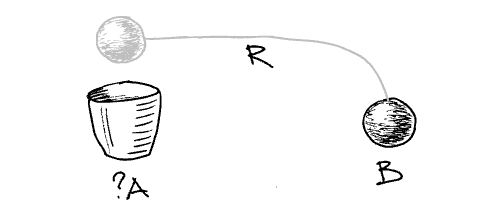
\includegraphics[width=0.6\linewidth]{chapter/bucketsAndBalls/graphPattern.PNG}
\end{figure*}

Корзина \textbf{?A} должна быть заполнена теми мячами, которые имеют отношение \textbf{R} к мячу \textbf{B}.

Но это выглядит лучше, если мы сокращаем его так:
\begin{figure*}[h]
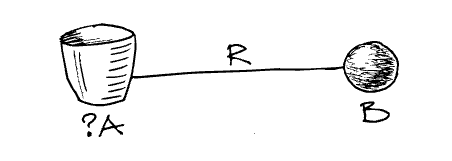
\includegraphics[width=0.6\linewidth]{graphics/chapter/bucketsAndBalls/graphPatternBucketsBalls.PNG}
\end{figure*}

Это шаблон графика в нотации <<Корзины и мячи>>. Направление отношения R не показано, но оно всегда слева направо.

Затем процесс написания и выполнения запроса SPARQL будет состоять из следующих этапов:
\begin{enumerate}
    \item Выберите свои корзины (в них вы собираетесь набирать нужные вам мячи).
    \item Составьте свои условия в виде графа корзин и мячей.
    \item Запустите свой запрос, чтобы заполнить ваши корзины мячами.
\end{enumerate}
